\documentclass[12pt,letterpaper,fleqn]{hmcpset}
\usepackage[margin=1in]{geometry}
\usepackage{graphicx}
\usepackage{amsmath,amssymb}
\usepackage{enumerate}
\usepackage{hyperref}
\usepackage{parskip}

% Theorems
\usepackage{amsthm}
\renewcommand\qedsymbol{$\blacksquare$}
\makeatletter
\@ifclassloaded{article}{
    \newtheorem{definition}{Definition}[section]
    \newtheorem{example}{Example}[section]
    \newtheorem{theorem}{Theorem}[section]
    \newtheorem{corollary}{Corollary}[theorem]
    \newtheorem{lemma}{Lemma}[theorem]
}{
}
\makeatother

% Random Stuff
\setlength\unitlength{1mm}

\newcommand{\insertfig}[3]{
\begin{figure}[htbp]\begin{center}\begin{picture}(120,90)
\put(0,-5){\includegraphics[width=12cm,height=9cm,clip=]{#1.eps}}\end{picture}\end{center}
\caption{#2}\label{#3}\end{figure}}

\newcommand{\insertxfig}[4]{
\begin{figure}[htbp]
\begin{center}
\leavevmode \centerline{\resizebox{#4\textwidth}{!}{\input
#1.pstex_t}}
\caption{#2} \label{#3}
\end{center}
\end{figure}}

\long\def\comment#1{}

\newcommand\norm[1]{\left\lVert#1\right\rVert}
\DeclareMathOperator*{\argmin}{arg\,min}
\DeclareMathOperator*{\argmax}{arg\,max}

% bb font symbols
\newfont{\bbb}{msbm10 scaled 700}
\newcommand{\CCC}{\mbox{\bbb C}}

\newfont{\bbf}{msbm10 scaled 1100}
\newcommand{\CC}{\mbox{\bbf C}}
\newcommand{\PP}{\mbox{\bbf P}}
\newcommand{\RR}{\mbox{\bbf R}}
\newcommand{\QQ}{\mbox{\bbf Q}}
\newcommand{\ZZ}{\mbox{\bbf Z}}
\renewcommand{\SS}{\mbox{\bbf S}}
\newcommand{\FF}{\mbox{\bbf F}}
\newcommand{\GG}{\mbox{\bbf G}}
\newcommand{\EE}{\mbox{\bbf E}}
\newcommand{\NN}{\mbox{\bbf N}}
\newcommand{\KK}{\mbox{\bbf K}}
\newcommand{\KL}{\mbox{\bbf KL}}

% Vectors
\renewcommand{\aa}{{\bf a}}
\newcommand{\bb}{{\bf b}}
\newcommand{\cc}{{\bf c}}
\newcommand{\dd}{{\bf d}}
\newcommand{\ee}{{\bf e}}
\newcommand{\ff}{{\bf f}}
\renewcommand{\gg}{{\bf g}}
\newcommand{\hh}{{\bf h}}
\newcommand{\ii}{{\bf i}}
\newcommand{\jj}{{\bf j}}
\newcommand{\kk}{{\bf k}}
\renewcommand{\ll}{{\bf l}}
\newcommand{\mm}{{\bf m}}
\newcommand{\nn}{{\bf n}}
\newcommand{\oo}{{\bf o}}
\newcommand{\pp}{{\bf p}}
\newcommand{\qq}{{\bf q}}
\newcommand{\rr}{{\bf r}}
\renewcommand{\ss}{{\bf s}}
\renewcommand{\tt}{{\bf t}}
\newcommand{\uu}{{\bf u}}
\newcommand{\ww}{{\bf w}}
\newcommand{\vv}{{\bf v}}
\newcommand{\xx}{{\bf x}}
\newcommand{\yy}{{\bf y}}
\newcommand{\zz}{{\bf z}}
\newcommand{\0}{{\bf 0}}
\newcommand{\1}{{\bf 1}}

% Matrices
\newcommand{\Ab}{{\bf A}}
\newcommand{\Bb}{{\bf B}}
\newcommand{\Cb}{{\bf C}}
\newcommand{\Db}{{\bf D}}
\newcommand{\Eb}{{\bf E}}
\newcommand{\Fb}{{\bf F}}
\newcommand{\Gb}{{\bf G}}
\newcommand{\Hb}{{\bf H}}
\newcommand{\Ib}{{\bf I}}
\newcommand{\Jb}{{\bf J}}
\newcommand{\Kb}{{\bf K}}
\newcommand{\Lb}{{\bf L}}
\newcommand{\Mb}{{\bf M}}
\newcommand{\Nb}{{\bf N}}
\newcommand{\Ob}{{\bf O}}
\newcommand{\Pb}{{\bf P}}
\newcommand{\Qb}{{\bf Q}}
\newcommand{\Rb}{{\bf R}}
\newcommand{\Sb}{{\bf S}}
\newcommand{\Tb}{{\bf T}}
\newcommand{\Ub}{{\bf U}}
\newcommand{\Wb}{{\bf W}}
\newcommand{\Vb}{{\bf V}}
\newcommand{\Xb}{{\bf X}}
\newcommand{\Yb}{{\bf Y}}
\newcommand{\Zb}{{\bf Z}}

% Calligraphic
\newcommand{\Ac}{{\cal A}}
\newcommand{\Bc}{{\cal B}}
\newcommand{\Cc}{{\cal C}}
\newcommand{\Dc}{{\cal D}}
\newcommand{\Ec}{{\cal E}}
\newcommand{\Fc}{{\cal F}}
\newcommand{\Gc}{{\cal G}}
\newcommand{\Hc}{{\cal H}}
\newcommand{\Ic}{{\cal I}}
\newcommand{\Jc}{{\cal J}}
\newcommand{\Kc}{{\cal K}}
\newcommand{\Lc}{{\cal L}}
\newcommand{\Mc}{{\cal M}}
\newcommand{\Nc}{{\cal N}}
\newcommand{\Oc}{{\cal O}}
\newcommand{\Pc}{{\cal P}}
\newcommand{\Qc}{{\cal Q}}
\newcommand{\Rc}{{\cal R}}
\newcommand{\Sc}{{\cal S}}
\newcommand{\Tc}{{\cal T}}
\newcommand{\Uc}{{\cal U}}
\newcommand{\Wc}{{\cal W}}
\newcommand{\Vc}{{\cal V}}
\newcommand{\Xc}{{\cal X}}
\newcommand{\Yc}{{\cal Y}}
\newcommand{\Zc}{{\cal Z}}

% Bold greek letters
\newcommand{\alphab}{\hbox{\boldmath$\alpha$}}
\newcommand{\betab}{\hbox{\boldmath$\beta$}}
\newcommand{\gammab}{\hbox{\boldmath$\gamma$}}
\newcommand{\deltab}{\hbox{\boldmath$\delta$}}
\newcommand{\etab}{\hbox{\boldmath$\eta$}}
\newcommand{\lambdab}{\hbox{\boldmath$\lambda$}}
\newcommand{\epsilonb}{\hbox{\boldmath$\epsilon$}}
\newcommand{\nub}{\hbox{\boldmath$\nu$}}
\newcommand{\mub}{\hbox{\boldmath$\mu$}}
\newcommand{\zetab}{\hbox{\boldmath$\zeta$}}
\newcommand{\phib}{\hbox{\boldmath$\phi$}}
\newcommand{\psib}{\hbox{\boldmath$\psi$}}
\newcommand{\thetab}{\hbox{\boldmath$\theta$}}
\newcommand{\taub}{\hbox{\boldmath$\tau$}}
\newcommand{\omegab}{\hbox{\boldmath$\omega$}}
\newcommand{\xib}{\hbox{\boldmath$\xi$}}
\newcommand{\sigmab}{\hbox{\boldmath$\sigma$}}
\newcommand{\pib}{\hbox{\boldmath$\pi$}}
\newcommand{\rhob}{\hbox{\boldmath$\rho$}}

\newcommand{\Gammab}{\hbox{\boldmath$\Gamma$}}
\newcommand{\Lambdab}{\hbox{\boldmath$\Lambda$}}
\newcommand{\Deltab}{\hbox{\boldmath$\Delta$}}
\newcommand{\Sigmab}{\hbox{\boldmath$\Sigma$}}
\newcommand{\Phib}{\hbox{\boldmath$\Phi$}}
\newcommand{\Pib}{\hbox{\boldmath$\Pi$}}
\newcommand{\Psib}{\hbox{\boldmath$\Psi$}}
\newcommand{\Thetab}{\hbox{\boldmath$\Theta$}}
\newcommand{\Omegab}{\hbox{\boldmath$\Omega$}}
\newcommand{\Xib}{\hbox{\boldmath$\Xi$}}

% mixed symbols
\newcommand{\sinc}{{\hbox{sinc}}}
\newcommand{\diag}{{\hbox{diag}}}
\renewcommand{\det}{{\hbox{det}}}
\newcommand{\trace}{{\hbox{tr}}}
\newcommand{\tr}{\trace}
\newcommand{\sign}{{\hbox{sign}}}
\renewcommand{\arg}{{\hbox{arg}}}
\newcommand{\var}{{\hbox{var}}}
\newcommand{\cov}{{\hbox{cov}}}
\renewcommand{\Re}{{\rm Re}}
\renewcommand{\Im}{{\rm Im}}
\newcommand{\eqdef}{\stackrel{\Delta}{=}}
\newcommand{\defines}{{\,\,\stackrel{\scriptscriptstyle \bigtriangleup}{=}\,\,}}
\newcommand{\<}{\left\langle}
\renewcommand{\>}{\right\rangle}
\newcommand{\Psf}{{\sf P}}
\newcommand{\T}{\top}
\newcommand{\m}[1]{\begin{bmatrix} #1 \end{bmatrix}}


% info for header block in upper right hand corner
\name{}
\class{Math189R SP19}
\assignment{Homework 4}
\duedate{Monday, Feb 25, 2019}

\begin{document}


\begin{problem}[1]
\textbf{(Conditioning a Gaussian)} Note that from Murphy page 113. ``Equation 4.69
is of such importance in this book that we have put a box around it, so you can easily
find it.'' That equation is important. Read through the proof of the result.
Suppose we have a distribution over random variables $\xx = (\xx_1, \xx_2)$ that is
jointly Gaussian with parameters
\[
    \mub = \m{\mub_1\\\mub_2}\;\;\; \Sigmab = \m{\Sigmab_{11}&\Sigmab_{12}\\\Sigmab_{21}&\Sigmab_{22}},
\]
where
\[
    \mub_1 = \m{0\\0}, \;\; \mub_2 = 5, \;\; \Sigmab_{11} = \m{6 & 8\\ 8 & 13}, \;\; \Sigmab_{21}^\T = \Sigmab_{12} = \m{5\\11}, \;\; \Sigmab_{22} = \m{14}.
\]
Compute
\begin{enumerate}[(a)]
    \item The marginal distribution $p(\xx_1)$.
    \item The marginal distribution $p(\xx_2)$.
    \item The conditional distribution $p(\xx_1 | \xx_2)$
    \item The conditional distribution $p(\xx_2 | \xx_1)$
\end{enumerate}

\end{problem}
\begin{solution}
\begin{enumerate}[(a)]
    \item $$p(x_1) = \mathcal{N}(\mu_{1}, \Sigma_{11}) = \mathcal{N} \left( \begin{bmatrix} 0 \\ 0 \end{bmatrix}, \begin{bmatrix} 6 & 8 \\ 8 & 13 \end{bmatrix} \right)$$
    \item $$p(x_2) = \mathcal{N}(\mu_2, \Sigma_{22}) = \mathcal{N}(5, 14)$$

    \item Note we can find $$\mu_{12} = \mu_1 + \Sigma_{12}\Sigma_{22}^{-1}(x_2 - \mu_2) = \frac{1}{14} \begin{bmatrix} 5 \\ 11 \end{bmatrix} (x_2 - 5)$$

$$\Sigma_{12} = \Sigma_{11} - \Sigma_{12}\Sigma_{22}^{-1}\Sigma_{21} = \begin{bmatrix} 6 & 8 \\ 8 & 13 \end{bmatrix} - \frac{1}{14} \begin{bmatrix} 5 \\ 11 \end{bmatrix} \begin{bmatrix} 5 & 11 \end{bmatrix} = \begin{bmatrix} \frac{59}{14} & \frac{57}{14} \\ \frac{57}{14} & \frac{61}{14} \end{bmatrix}.$$
Then, $$p(x_1|x_2) = \mathcal{N} (\mu_{12}, \Sigma_{12})
 = \mathcal{N}\left(\frac{1}{14} \begin{bmatrix} 5 \\ 11 \end{bmatrix} (x_2 - 5),  \begin{bmatrix} \frac{59}{14} & \frac{57}{14} \\ \frac{57}{14} & \frac{61}{14} \end{bmatrix}\right)$$
 
	\item Similar to part c, we can find $$\mu_{21} = \mu_2 + \Sigma_{21}\Sigma_{11}^{-1}(x_1 - \mu_1) = 5 + \begin{bmatrix} 5 & 11 \end{bmatrix} \begin{bmatrix} 6 & 8 \\ 8 & 13 \end{bmatrix}^{-1} (x_1 - \mu_1) = 5 + \frac{1}{14} \begin{bmatrix} 23 & 13 \end{bmatrix} x_1$$

$$\Sigma_{21} = \Sigma_{22} - \Sigma_{21}\Sigma_{11}^{-1}\Sigma_{12} = 14 - \begin{bmatrix} 5 & 11 \end{bmatrix} \begin{bmatrix} 6 & 8 \\ 8 & 13 \end{bmatrix}^{-1} \begin{bmatrix} 5 \\ 11 \end{bmatrix} = \frac{25}{14}.$$
Then, $$p(x_2|x_1) = \mathcal{N} (\mu_{21}, \Sigma_{21})=\mathcal{N}\left(5 + \frac{1}{14} \begin{bmatrix} 23 & 13 \end{bmatrix} x_1, \frac{25}{14}\right).
$$

\end{enumerate}
\end{solution}
\newpage

\begin{problem}[2]
(\textbf{MNIST}) 
In this problem, we will use the MNIST dataset, a classic in the deep learning literature as a toy dataset to test
algorithms on, to set up a model for logistic regression and softmax regression. In the starter code, we have already parsed the data for you. However, you might need internet connection to access the data and therefore successfully run the starter code.
\newline
\newline
The problem is this: we have images of handwritten
digits with $28\times 28$ pixels in each image, as well as the label of which digit $0 \leq \texttt{label} \leq 9$ the written
digit corresponds to. Given a new image of a handwritten digit, we want to be
able to predict which digit it is.
The format of the data is \texttt{label, pix-11, pix-12, pix-13, ...}
where \texttt{pix-ij} is the pixel in the \texttt{ith} row and \texttt{jth} column.
\newline
\begin{enumerate}[(a)]
    \item (\textbf{logistic}) Restrict the dataset to only the digits with a label
        of 0 or 1. Implement L2 regularized logistic regression as a model to compute
        $\PP(y=1|\xx)$ for a different value of the regularization parameter $\lambda$.
        Plot the learning curve (objective vs. iteration) when using Newton's Method
        \textit{and} gradient descent.
        Plot the accuracy, precision ($p = \PP(y=1 | \hat y=1)$), recall ($r = \PP(\hat y=1 | y=1)$),
        and F1-score ($F1 = 2pr / (p+r)$) for different values of $\lambda$ (try at least
        10 different values including $\lambda = 0$) on the test set and report the
        value of $\lambda$ which maximizes the accuracy on the test set. What is your
        accuracy on the test set for this model? Your accuracy should definitely be
        over 90\%.

    \item (\textbf{softmax}) Now we will use the whole dataset and predict the label
        of each digit using L2 regularized softmax regression (multinomial logistic
        regression). Implement this using gradient descent, and plot the accuracy
        on the test set for different values of $\lambda$, the regularization parameter.
        Report the test accuracy for the optimal value of $\lambda$ as well as it's
        learning curve. Your accuracy should be over 90\%.

\end{enumerate}
\end{problem}
\newpage
\begin{solution}
\begin{enumerate}[(a)]
	\item Here are the resulting plots.
	
	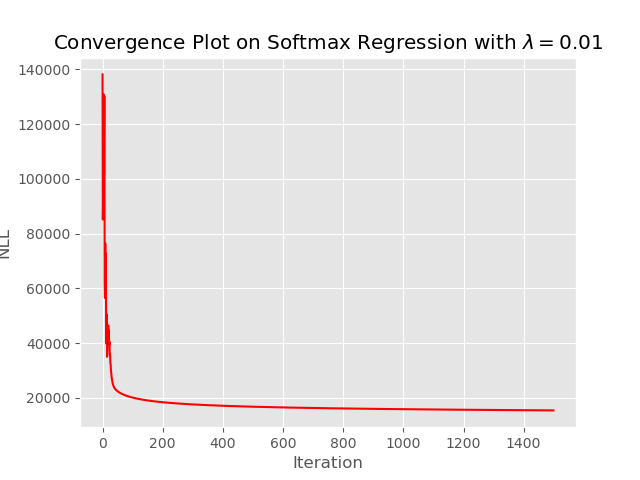
\includegraphics[scale=0.5]{hw4pr2b_convergence.png}
	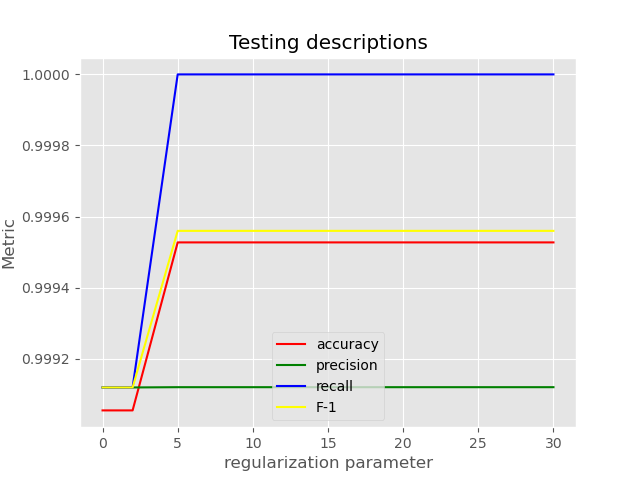
\includegraphics[scale=0.5]{hw4pr2a_description.png}
	As we can see from above, our accuracy is around 0.995.
	
	\item Here are the resulting plots.
	
	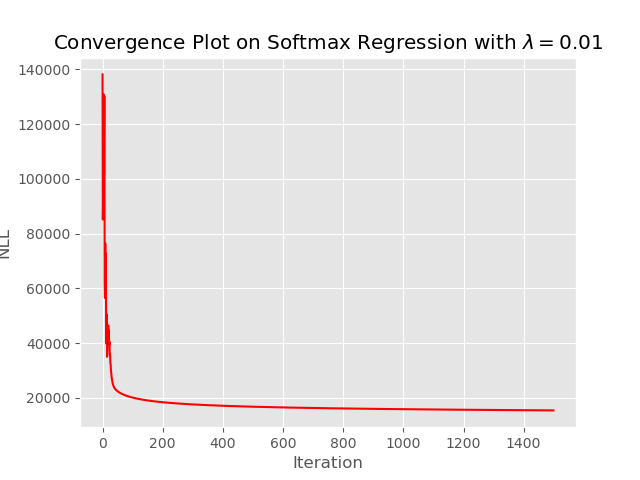
\includegraphics[scale=0.5]{hw4pr2b_convergence.png}
	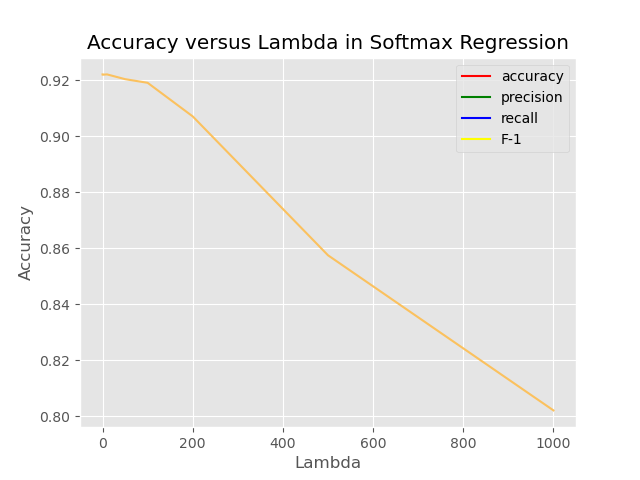
\includegraphics[scale=0.5]{hw4pr2b_lva.png}
	 
	As we can see from above, our accuracy is around 0.92
\end{enumerate}
\end{solution}
\newpage

\end{document}
